% ------ Clase de documento ------
\documentclass[a4paper,10pt,oneside]{article}

%-------------------------------------Paquetes-----------------------------------------------------------------------
\usepackage[spanish]{babel}  % Traduce los textos a castellano
\usepackage[utf8]{inputenc}	% Permite escribir directamente áéíóúñ
\usepackage{t1enc}            	% Agrega caracteres extendidos al font
\usepackage{amsmath} 		%Permite imprimir mas opcciones matematicas
\usepackage{graphicx}		%Permite agregar imagenes al informe
\usepackage{multicol}  		%Permite dividir el texto en varias columnas
\usepackage{anysize}		%Permite modificar los margenes del documento
\usepackage{float} 			%Permite utilizar H para colocar las imagenes en un lugar especifico 
\usepackage{multirow}		%Permite dividir las tablas en subtablas
\usepackage{booktabs}		%Permiten manejar mejor el tamaño de las tablas
\usepackage{tabulary}		%Permiten manejar mejor el tamaño de las tablas
\usepackage{fancyhdr}		%Permite agregar encabezado y pie fancy

\usepackage{courier}		%
\usepackage{color}			%
\usepackage{listings}  		%Permite agregar codigo directamente sobre el documento

%---------------------------------------Definiciones propias---------------------------------------------------------
\newcommand{\grad}{\hspace{-2mm}$\phantom{a}^{\circ}$} %El º que no existe como comando
\newcommand{\oiint}{\displaystyle\bigcirc\!\!\!\!\!\!\!\!\int\!\!\!\!\!\int} %Integral doble cerrada
%------------------------------------------------------------------------------------------------------------------------

%-------------------------------------Configuracion De Codigo----------------------------------
\definecolor{dkgreen}{rgb}{0,0.6,0}
\definecolor{gray}{rgb}{0.5,0.5,0.5}

\lstset{language=C,
	breaklines=true,
	keywordstyle=\bf\color{blue},
	commentstyle=\tt\it\color{dkgreen},
	stringstyle=\color{gray},
 	numbers=left,
	numberstyle=\tiny\color{black},
	stepnumber=2,
	numbersep=8pt,
	backgroundcolor=\color{white},
	tabsize=4,
	showspaces=false,
	showstringspaces=false}

\newcommand{\captionlisting}[2][]{%
    \lstinputlisting[caption={\large{\detokenize{#2}}},#1]{#2}%
}

\renewcommand\lstlistingname{Archivo}
%%%%%%%%%%%%%%%%%%%%%%%%%%%%%%%%%%%%%%%%%%%%%%%%%%%

% ------ Configuración ------
\title{\textbf{66.20 Organización de Computadoras\\ Trabajo Práctico 0: \\ Infraestructura básica}}

\author{	Burdet Rodrigo, \textit{Padrón Nro. 93440}\\
            \texttt{ rodrigoburdet@gmail.com}\\\\
            Romani Nazareno, \textit{Padrón Nro. 83991}                     \\
            \texttt{ nazareno.romani@gmail.com}\\\\
            Martinez Gaston Alberto, \textit{Padrón Nro. 91383}                     \\
            \texttt{ gaston.martinez.90@gmail.com }\\\\[2.5ex]
            \normalsize{1er. Cuatrimestre de 2014}                       \\
            \normalsize66.20 Organización de Computadoras\\
            \normalsize{Facultad de Ingeniería, Universidad de Buenos Aires}            \\
       }
\date{\today}



% ----- Cuerpo del documento -----
\begin{document}
\maketitle

\thispagestyle{empty}

\newpage

\section{Objetivos}
    Familiarizarse con las herramientas de software que usaremos en los siguientes trabajos, implementando un programa (y su correspondiente documentación) que resuelva el problema piloto que presentaremos mas abajo.

\section{Resumen}
    En el presente trabajo, se implementó un algoritmo que resuelve la transformación de un conjunto arbitrario de bytes en un conjunto formado por caracteres ASCII y viceversa. Los distintos valores a codificar/decodificar,  son obtenidos a través de los parámetros definidos en el enunciado.
    El programa fue compilado tanto en la máquina host (sistema operativo Linux), como en una máquina corriendo el sistema operativo NetBSD.

\section{Desarrollo}
	
\subsection{Paso 1: Configuración de Entorno de Desarrollo}
El primer paso fue configurar el entorno de desarrollo, de acuerdo a la guía facilitada por la cátedra. \\
Trabajamos con una distribución de Linux basada en Debian y con el GxEmul proporcionado por la cátedra, el cual tiene ya configurado NetBSD.
	
\subsection{Paso 2: Implementación del programa}
El programa debe ejecutarse por línea de comando y la salida del mismo dependerá del valor de los argumentos con los que se lo haya invocado.
\subsubsection{Ingreso de parámetros}
El formato para invocar al programa es el siguiente:
\begin{center}
	\texttt{./tp0 [OPTIONS]}
\end{center}
Los parámetros válidos que puede recibir el programa son los siguientes: \\ 

\begin{ttfamily}
\begin{tabular}{lll}

\bf{-e,} & \bf{--encode} &(Encodes to Base64). \\
\bf{-d,} & \bf{--decode} &(Decodes from Base64).\\
\bf{-i,} & \bf{--input file} &(Reads from file or stdin).\\
\bf{-o,} & \bf{--output file} &(Writes to file or stdout).\\
\bf{-v,} & \bf{--version} 	&(Show version string).\\
\bf{-h,} & \bf{--help} &(Print this message and quit).\\
\end{tabular}
\end{ttfamily}

\subsubsection{Interpretación de parámetros}
Para parsear los parámetros se usaron las funciones definidas en arg\_parse.h. Se puede conocer más en detalle el funcionamiento de las mismas, a través de la documentación incluida en dicho archivo. 
		Estas funciones permiten recoger los parámetros de entrada del programa y ejecutar la funcionalidad correspondiente. Estas son compatibles con NetBSD.
			
	\section{Compilación del programa}
	
	Para poder compilar el proyecto, se debe abrir una terminal Linux dentro del directorio donde se encuentra el código 
	fuente escrito en C, y ejecutar el script \textit{Makefile} con el comando \texttt{make} \footnote{Requiere tener instalado el programa \it{Make} y el compilador \it{GCC}}. Este comando ejecuta las directivas definidas en el archivo \texttt{Makefile} generado para tal caso. 
		
	 Esto generara un archivo ejecutable, llamado \textit{tp0} \footnote{El nombre del ejecutable se puede editar desde el script o desde la consola al invocar \texttt{make}}.  Tambien se puede ejecutar el comando \texttt{make Valgrind} para compilar el programa y correrlo con \textit{Valgrind}, de manera de poder depurarlo en modo interactivo.
		 
	\section{Compilación del programa en NetBSD}
	
	Para poder compilar el proyecto en NetBSD, se debe ejecutar el comando:
	
	\begin{center}
	\texttt{Gcc -c -S -O0 -mrnames arg_parse.c base_64.c main.c} 
	\end{center}
	
	
\section{Corridas de prueba y Mediciones}

	En las figuras que siguen a continuación se muestran los comandos utilizados para ejecutar el programa y se puede apreciar los resultados de las diferentes pruebas que realizamos. Cabe acotar que cuando se encodea un archivo( \texttt{./tp0 -e -i <archivo>}), también se encodea el fin del mismo. \newpage
	
	\begin{figure}[H]
		\begin{center}
			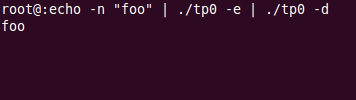
\includegraphics[width=0.50\textwidth]{test1.png}
		\end{center}
		\caption{Codificación de texto `foo`} \label{Figura 1}
	\end{figure}

	\begin{figure}[H]
		\begin{center}
			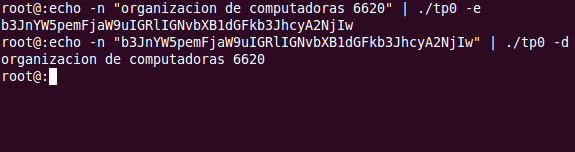
\includegraphics[width=0.80\textwidth]{test2.png}
		\end{center}
		\caption{Codificación/Decodificación de texto `organizacion de computadoras 6620`} \label{Figura 2}
	\end{figure}

	\begin{figure}[H]
		\begin{center}
			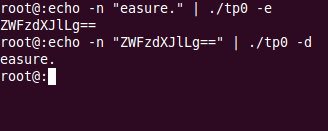
\includegraphics[width=0.50\textwidth]{test3.png}
		\end{center}
		\caption{Codificación/Decodificación de texto con uso de caracter de padding} \label{Figura 3}
	\end{figure}
	
	\begin{figure}[H]
		\begin{center}
			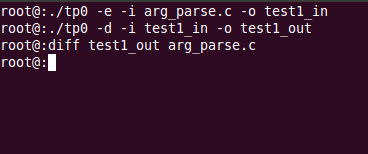
\includegraphics[width=0.50\textwidth]{test4.png}
		\end{center}
		\caption{Codificación a través de archivo de entrada guardando la salida en otro archivo, decodificación de este último y comparación de archivos} \label{Figura 4}
	\end{figure}
	
	\newpage
\appendix
\section{Codigo C}

\captionlisting{../arg_parse.h}
\captionlisting{../arg_parse.c}

\captionlisting{../base_64.h}
\captionlisting{../base_64.c}

\captionlisting{../main.c}
\newpage
\section{Makefile}

\lstinputlisting[language=make,
			breaklines=true,
			keywordstyle=\bf\color{blue},
			commentstyle=\tt\it\color{dkgreen},
			stringstyle=\color{gray},
 			numbers=left,
			numberstyle=\tiny\color{black},
			stepnumber=1,
			numbersep=8pt,
			backgroundcolor=\color{white},
			tabsize=4,
			showspaces=false,
			showstringspaces=false]{../Makefile}

\newpage
\section{Conclusiones}	
	Como se enuncia en el objetivo de este trabajo práctico, aprendimos a instalar y manejar el GxEmul, a realizar transferencias de archivos en Linux, así como también compilar y ejecutar programas en el NetBSD. Por otro lado,  aprendimos a manejar y escribir informes en \LaTeX{}.
	De este modo, estamos preparados para que en los próximos trabajos prácticos, nos aboquemos directamente al desarrollo de los mismos.

\end{document}

